\section{How the experiments measure progress}\label{sec:measurement}

The most consequential methodological change is the movement from a
headline counter to a complete, explicit accounting boundary. The same
research direction can look favourable when only relation probes are
counted, unfavourable when each probe is priced, and different again when
setup and linear algebra are included. The programme's rules were written
in response to concrete examples of this failure mode.\src{C-RULES}
\src{RESIDUAL}

\subsection{Cost boundaries and comparable units}

The historical normalisation is
\[
 S=\frac{\text{total charged group-addition-equivalent work}}{\sqrt r}.
\]
Within an explicit curve, subgroup and implementation, this makes a
square-root generic reference roughly flat. It does not make different
primitive weights, memory envelopes or target laws interchangeable. Some
studies count field multiplications, some Boolean word XORs, some
simulated instructions, and some admitted wall time. A conversion must be
measured or explicitly modelled before units can be joined.

A cold solve includes reusable setup, factor-base construction, indexes,
relation collection, matrix work, target work and verification. An online
solve starts after reusable state has been prepared and excludes that
state's construction. Both questions are useful. The online question
requires a comparator with the same advice and reuse opportunity; the
cold question requires setup on both arms. A ratio between IC cold
process time and rho online time can be recorded as a diagnostic, but is
not a matched cold method ratio.

The current one-target contract also separates target-dependent phases.
It disallows replacing a one-target rho reference with a multi-target
batch, or dividing a shared collision search by target count and calling
the result one-target latency. Repeated one-target workloads form a panel;
they do not become a single batch ECDLP simply because the statistics are
computed together.\src{C-RULES}\src{N83}

\subsection{Unpriced work and the sensitivity band}

Many historical counters omit native operations. Rho can omit
canonicalisations, partition hashes and table operations; IC can omit
root calls, native matrix work or membership tests. If $L_A\le C_A$ and
$L_B\le C_B$ are incomplete cost lower bounds, then $L_A/L_B$ does not
bound $C_A/C_B$ in either direction. A ratio of lower bounds is not a
lower bound on the ratio.

The October accounting rule therefore prices emitted unpriced operations
at several common weights, including $w\in\{0,0.1,1\}$ GAE, on all arms.
A ranking is accepted only if it survives the band. A missing counter
emission cannot be repaired by choosing a weight: it remains an
implementation gap. A pinned primitive calibration can supplement the
band but cannot silently replace it on one side only.\src{C-RULES}

The band is a sensitivity analysis, not a claim that a 64-bit XOR and a
hash-table lookup really have identical cost. This is especially visible
for F4: weighting every XOR at 0.1 GAE is much more expensive than one
study's pinned calibration near 0.002 GAE. The conservative conclusion
must state where it depends on the band or on a particular calibration.
\src{FRONTIER}

\subsection{From exploratory scripts to sealed records}

The record includes exploratory scripts, toy known-answer ladders,
Autolab tournaments, immutable experiment contracts, ICMS and ecbench
sessions, native compiler and emulator checks, hardware experiments,
and independent replay receipts. The ecbench instruments add explicit
specifications, method and workload identities, per-run outcomes, source
and binary hashes, host manifests, cost phases, replay audits and
comparison records. The SQLite index is a view of evidence, not a
substitute for the sealed evidence.

Earlier scripts remain useful historical observations. They do not
automatically meet newer isolation, primary-online-window or replay
contracts. In particular, the migration of a result into a dashboard
cannot improve its evidence tier. The research orchestrator likewise
separates an executor's observation from a coordinator's official status
transition and an independent review.\src{AR-README}\src{C-RULES}

\subsection{Controls and statistical design}

Several recurring practices are worth retaining: freeze the protocol
before the measurement; tune on disjoint training points; test on held-out
public points; interleave arms; include identical A/A controls; verify
every returned scalar or root set; retain failures; and bootstrap over the
actual independent workload or curve unit. Five targets are not 25
independent targets merely because five configurations ran on each.
Similarly, repeat-bootstrap intervals on one scalar panel do not become
coverage over arbitrary scalar distributions.

Positive controls show that an instrument can detect the proposed kind of
signal; null controls show whether the same apparent signal arises without
the mechanism. The ML studies use class-held-out splits and label
permutation; decomposition studies compare with exhaustive point sums;
GPU studies compare ranks and pinned variables across paths. A failed
control is retained even when the main result appears favourable.

Resource failures are a separate outcome. Exhaustion means the declared
search budget ended. A timeout or memory cap says something about the
specific execution, not nonexistence of the desired relation. A failed
artifact-integrity gate can make a run inadmissible without supplying
negative evidence about the mathematics.

\subsection{A freshly checked campaign}

The 15 October frontier campaign is a stronger common reference than a
collection of unrelated best cells. Its 19 sessions cover eight Koblitz
curves, six NIST-shaped prime curves and five prime Kummer-ladder curves,
with 16 public targets, two measured rounds and a warm-up. The sessions
contain 4,848 executions: 4,769 verified and 79 exhausted including
warm-ups. Removing warm-ups leaves 3,232 measured executions: 3,178
verified and 54 exhausted. Every stored record-file hash matches its
session manifest in this review. The stored audits contain 3,178
successful identical replays of verified measured records; exhausted
records are retained separately, not reported as successful replays.
\src{FRONTIER}\src{BAND}

No IC arm in that campaign beats the cheapest matched constant-memory
rho arm at any of the three band weights. Compact-orbit IC is closest on
the Koblitz ladder: its IC/rho ratio is 3.8--15.0 with the extra native
work priced at zero, and 4.9--17.8 at $w=0.1$. Prime pair-table IC grows
from approximately 10.5 to 101.8 times rho at $w=0.1$ over the
20--40-bit ladder. The campaign's fitted exponent differences are not
uniformly separated at every weight. This establishes a bounded
comparison on those implementations and instances, not a theorem that all
future IC must lose.

\begin{figure}[htbp]
\centering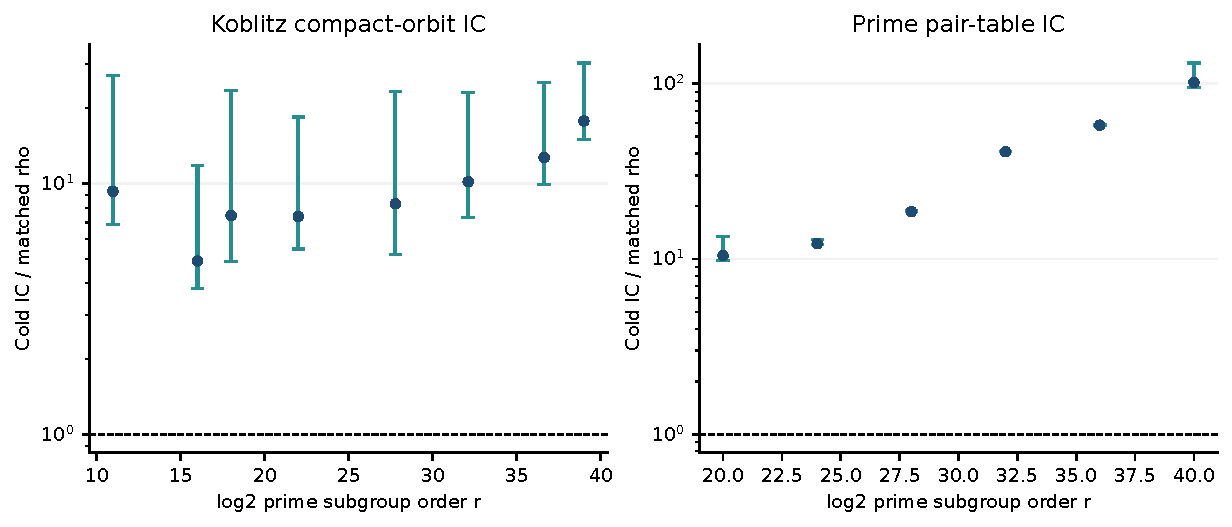
\includegraphics[width=\linewidth]{figures/frontier.pdf}
\caption{The campaign's recorded cold IC/rho ratios. The centre marks
$w=0.1$; the spans show $w=0$ through $w=1$. Every displayed cell has
32 verified measured runs. These are counted-work comparisons at L0,
not new native wall-time measurements. Koblitz points are ordered by
subgroup size, which need not follow field degree. Source: \src{BAND}.}
\label{fig:frontier}
\end{figure}

The campaign does not supersede every later experiment. Its role is a
fixed, comparatively well-accounted baseline. Later improvements require
their own matched comparison before being used to move this frontier.

\subsection{Corrections as an experimental capability}

The programme now has repeated examples of a result being made less
favourable by better accounting: a relation-only crossover disappearing
after linear algebra was priced, F6 geometry dominating its saved XORs,
and online IC losing an advantage after rho was given preprocessing.
These are scientific corrections. They are also evidence that the
instruments can reject a preferred interpretation. They should remain in
the record beside the successful optimisations rather than being removed
from a progress narrative.
